\documentclass[italian]{article}
%\usepackage{fontspec}
\usepackage{tikz}
\usetikzlibrary{positioning}
\usetikzlibrary{arrows,decorations.pathreplacing}
\begin{document}
	
    \section*{Stato attuale dati trasmessi}
    
    \subsection*{keyboard}
    \begin{tabular}{ll}
        \texttt{pulsPFSE0001} & pfSense Halt \\
        \texttt{pulsPFSE0002} & pfSense Reboot \\
        \texttt{pulsPFSE0003} & pfSense Sync \\
        \texttt{pulsPFSE0004} & pfSense Ping \\
        \texttt{pulsACTU0001} & attuatore Rele ON\\
        \texttt{pulsACTU0002} & attuatore Rele OFF\\
        \texttt{pulsACTU0003} & attuatore leggi stato rele\\
        \texttt{pulsACTU0004} & attuatore leggi analogico A0\\            
    \end{tabular}
    
    \subsection*{servente}
    
    \begin{tabular}{ll}
        \texttt{statPFSE0000} & pfSense tentativo di sync Arduino-pfSense\\
        \texttt{statPFSE0001} & pfSense in avvio\\
        \texttt{statPFSE0002} & pfSense è ON\\
        \texttt{statPFSE0003} & pfSense in spegnimento\\
        \texttt{statPFSE0004} & pfSense è OFF \\
        \texttt{statPFSE0005} & pfSense ping OK\\
        \texttt{statPFSE0006} & pfSense pink ko\\
        \texttt{statPFSE0007} & pfSense ricevuto comando\\        

    \end{tabular}
    
    \subsection*{attuatore}    
    
    \begin{tabular}{ll}
        \texttt{digiACTU000X} & attuatore stato rele (X = [0/1])\\
        \texttt{anagACTU0XXX} & attuatore valore analogico A0 (X = [0/999])\\
        \texttt{statACTU0007} & attuatore ricevuto comando\\        
        
    \end{tabular}

\newpage
    
%	\section*{Principio di funzionamento}
%	
%	Il progetto viene sostanzialmente diviso in "funzioni": pulsantiera, display, attuatore.
	
    \subsection*{Dati}
    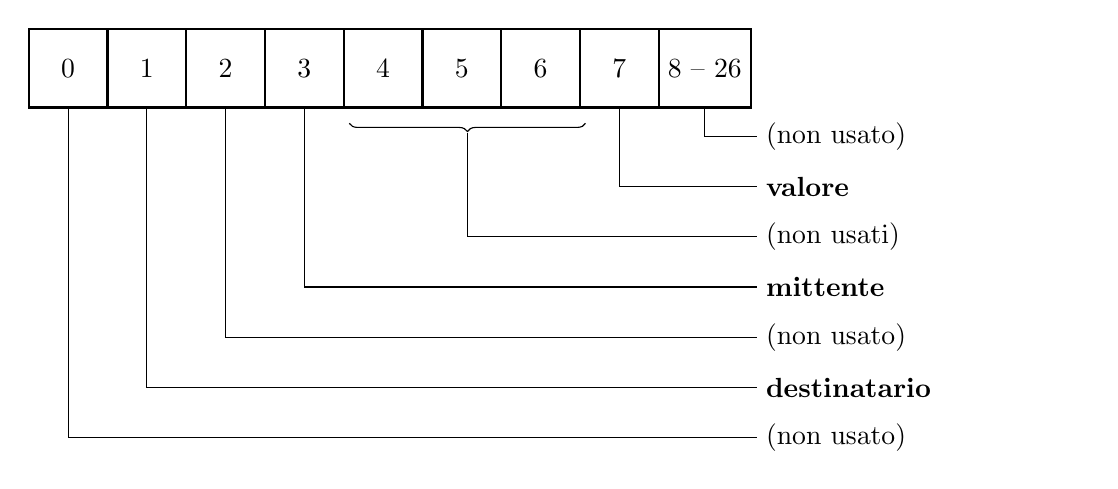
\begin{tikzpicture}[base/.style={draw,thick,minimum size=1cm,node distance=0pt,outer sep=0pt},altro/.style={text width=4cm,align=left,minimum size=0pt,node distance=3pt,outer sep=0pt}]
    \node[base](a){0};
    \node[base,right=of a,anchor=west](b){1};
    \node[base,right=of b,anchor=west](c){2};
    \node[base,right=of c,anchor=west](d){3};
    %
    \coordinate[yshift=-2mm,xshift=2pt](aa) at (d.south east);
    %
    \node[base,right=of d,anchor=west](e){4};
    \node[base,right=of e,anchor=west](f){5};
    \node[base,right=of f,anchor=west](g){6};
    \node[base,right=of g,anchor=west](h){7};                
    %
    \coordinate[yshift=-2mm,xshift=2pt](bb) at (h.south west);    
    %
    \node[base,right=of h,anchor=west](i){8 -- 26}; 
    %
    \node[altro,below right =of i,anchor=north west](x){(non usato)};
    \draw (i) |- (x);
    %
    \node[altro,below =of x](x){\textbf{valore}};
    \draw (h) |- (x);
    %
    \draw[decorate,decoration={brace,amplitude=3pt,mirror}] (aa) --  node(ww) {} (bb);        
    \node[altro,below =of x](x){(non usati)};
    \draw (ww) |- (x);
    %
    \node[altro,below =of x](x){\textbf{mittente}};
    \draw (d) |- (x);      
    %
    \node[altro,below =of x](x){(non usato)};
    \draw (c) |- (x);           
    %
    \node[altro,below =of x](x){\textbf{destinatario}};
    \draw (b) |- (x);      
    %
    \node[altro,below =of x](x){(non usato)};
    \draw (a) |- (x);               
    %

    \end{tikzpicture}
    
    \section*{Destinatario}
    
    Il byte è normalmente a zero (il messaggio viene inoltrato a tutti) ma se occorre fare in modo che il segnale venga ripetuto tra stazioni (esempio per comunicare tra appartamento e garage / cantina) si riempirà opportunamente questo campo.
    
    \section*{Mittente}
    
    Questo byte identifica nell'ambiente radio quale pulsante o risposta sta viaggiando nell'etere. Mantenendo aggiornata la tabella sottostante si semplifica la struttura software a discapito della flessibilità del sistema che sarà quindi altamente personalizzato.
    
    \subsection{Tabella mittenti/destinatari}
    
    

        \begin{tabular}{ll}
            \texttt{0} & tutti (broadcast): usato solo per destinatari\\
            %
            \multicolumn{2}{l}{\textbf{pulsantiera - inerente a pfSense}}\\
            % 
            \texttt{1} & Pulsante per spegnimento\\
            \texttt{2} & Pulsante per riavvio\\
            \texttt{3} & Pulsante per ping \\
            \texttt{4} & Pulsante sync \\
            \texttt{5} & Pulsante leggi stato (on/off/in accensione/in spegnimento)\\
            %
            \multicolumn{2}{l}{\textbf{pulsantiera - inerente a primo attuatore}}\\
            % 
            \texttt{6} & Pulsante accensione carico 01\\
            \texttt{7} & Pulsante spegnimento carico 01\\
            \texttt{8} & Pulsante lettura valore analogico canale A\\
			%
			\multicolumn{2}{l}{\textbf{pulsantiera - inerente a NAS}}\\
			% 
			\texttt{9} & Pulsante per spegnimento\\
			\texttt{10} & Pulsante per accensione\\
			\texttt{11} & Pulsante leggi stato (on/off/in accensione/in spegnimento)\\
			%
			\multicolumn{2}{l}{\textbf{pulsantiera - inerente a UPS}}\\
			% 
			\texttt{12} & Pulsante per spegnimento\\
			\texttt{13} & Pulsante per accensione\\
			\texttt{14} & Pulsante leggi stato (on/off)\\			
            %
            \multicolumn{2}{l}{\textbf{scheda server pfSense}}\\
            % 
            \texttt{30} & lettura stato pfSense (on/off/in accensione/in spegnimento)\\        
            \texttt{31} & lettura stato ping (connesso/non connesso a internet)\\            
            \texttt{32} & ricevuto il comando\\
            %
            \multicolumn{2}{l}{\textbf{primo attuatore}}\\
            % 
		    \texttt{40} & lettura stato logico carico 01\\ 
		    \texttt{41} & lettura valore analogico canale A\\
		    \texttt{42} & periodica lettura analogico canale A\\
			\texttt{43} & ricevuto il comando\\
			%
			\multicolumn{2}{l}{\textbf{scheda NAS}}\\
			\texttt{50} & lettura stato NAS (on/off/in accensione/in spegnimento)\\
			\texttt{51} & ricevuto il comando\\
			%
			\multicolumn{2}{l}{\textbf{scheda UPS}}\\
			\texttt{55} & lettura stato UPS (on/off)\\
			\texttt{56} & ricevuto il comando\\
			%
			\multicolumn{2}{l}{\textbf{ripetitori} (usati come destinatario o destinatario/mittente tra ripetitori)}\\
			%         
			\texttt{128} & ripetitore A\\    
			\texttt{129} & ripetitore B\\ 
        \end{tabular}

    \subsection*{Info}
    
    La scheda emette autonomamente questo valore: \'E compito della scheda display che sta in ascolto di avere "orecchie ben aperte". La risposta non dipende direttamente dallo stato di una uscita ma sono risposte in cascata.
    
    \section*{Valore}
    
    Questo byte può contenere un valore compreso tra 0 e 255
    
    \section*{Bytes non usati}
    
    Per applicazioni future. Ad esempio si possono sfruttare i bytes 4, 5, 6 e 7 per inviare un valore a 32 bit. E usare indirizzamenti a 16 bit. Al momento non implementato
    

	\subsection*{Pulsantiera}
	
	La pulsantiera manda nell'etere i dati relativi al pulsante trasmesso. Chi è in ascolto riceve il segnale e se è di sua competenza esegue l'azione richiesta relativa al pulsante che è stato premuto.
	
	La pulsantiera è anche in ascolto per capire se il comando è stato ricevuto. Se non è stato ricevuto lo ripete un certo numero di volte. In base alla risposta attiva un led verde oppure rosso. I led sono utili perché i pulsanti vengono fisicamente premuti da una persona che in questo modo può rendersi conto che il segnale è stato correttamente inoltrato.
	
	Di pulsantiere ce ne possono essere più di una, sia con stesse funzioni che con funzioni diverse.
	
	\bigskip
	
	\textbf{Nota:} non è compito della pulsantiera indicare lo stato di una uscita su un attuatore: Il led (unico sulla scheda della pulsantiera) indicherà unicamente la ricezione corretta del messaggio. Le altre informazioni saranno date dal display.
	
	\subsection*{Display}
	
	Il display visualizza quanto viene emesso nell'etere dagli attuatori. {\scriptsize Gli attuatori, che non sono presidiati, si accertano che il segnale venga ricevuto dal display, tentando un certo numero di volte la rispedizione del messaggio.}
	
	A sua volta il display potrà indicare indicherà il numero di minuti dall'ultima ricezione di ogni scheda-attuatore.
    
%    \subsubsection*{Ritardi nelle risposte}
%    
%    Di display ce ne possono essere più di uno con funzioni diverse. Quando un attuatore chiede conferma che un display abbia ricevuto il suo segnale .............. SAFOM? ......................
    
    \subsection*{Attuatore}
    
    Viene identificato come attuatore qualsiasi altra scheda che non sia una tastiera o un display. 
    
%    \section*{Dati trasmessi}
%    
%    Sono disponibili 24 bytes:
%    
%    \begin{itemize}
%        \item 2 byte per descrivere il tipo di oggetto
%        \item 2 byte per indicare l'ID dell'oggetto
%        \item 8 byte per il 'protocollo' del messaggio
%        \item 8 byte per un valore numerico
%        \item 1 byte per identificare un ripetitore
%        \item 3 bytes 'liberi' 
%    \end{itemize}
%    
%    \begin{tikzpicture}[base/.style={draw,thick,minimum size=0pt,node distance=0pt,outer sep=0pt},altro/.style={text width=4cm,align=left,minimum size=0pt,node distance=3pt,outer sep=0pt}]
%        \node[base](a){0};
%        \node[base,right=of a,anchor=west](b){1};
%        \node[base,right=of b,anchor=west](c){2};
%        \node[base,right=of c,anchor=west](d){3};
%        \node[base,right=of d,anchor=west](e){4 -- 11};
%        % aggiunti
%       
%        \node[base,right=of e,anchor=west](f){12 - 19};
%       
%        \node[base,right=of f,anchor=west](m){20}; 
%        \node[base,right=of m,anchor=west](n){21};
%        \node[base,right=of n,anchor=west](o){22};
%        \node[base,right=of o,anchor=west](p){23};                
%        %
%        \coordinate[yshift=-2mm,xshift=2pt](aa) at (a.south west);
%        \coordinate[yshift=-2mm,xshift=-2pt](bb) at (b.south east);
%        %
%        \coordinate[yshift=-2mm,xshift=2pt](cc) at (c.south west);
%        \coordinate[yshift=-2mm,xshift=-2pt](dd) at (d.south east);
%        %
%        \coordinate[yshift=-2mm,xshift=2pt](qq) at (e.south west);
%        \coordinate[yshift=-2mm,xshift=-2pt](rr) at (e.south east);
%        %
%        \coordinate[yshift=-2mm,xshift=2pt](ee) at (f.south west);
%        \coordinate[yshift=-2mm,xshift=-2pt](ll) at (f.south east);
%        %
%        \coordinate[yshift=-2mm,xshift=2pt](mm) at (m.south west);
%        \coordinate[yshift=-2mm,xshift=-2pt](pp) at (p.south west);        
%        %
%        \draw[decorate,decoration={brace,amplitude=3pt,mirror}] 
%        (aa) --  node(x) {} (bb);
%        \draw[decorate,decoration={brace,amplitude=3pt,mirror}] 
%        (cc) --  node(y) {} (dd);
%        \draw[decorate,decoration={brace,amplitude=3pt,mirror}] 
%        (ee) --  node(z) {} (ll);
%        \draw[decorate,decoration={brace,amplitude=3pt,mirror}] 
%        (mm) --  node(w) {} (pp);
%		 \draw[decorate,decoration={brace,amplitude=3pt,mirror}] 
%		 (qq) --  node(s) {} (rr);
%        %
%        
%        \node[altro,below right=of p,yshift=-10pt](sotto){ripetitore};
%        \draw (p) |- (sotto);
%        \node[altro,below=of sotto](sotto){\texttt{\begin{tabular}{ll}
%        		C & usa il ripetitore C\\
%        		\end{tabular}}};
%        
%        \node[altro,below =of sotto](sotto){non usati};
%        \draw (w) |- (sotto);
%                
%        
%        \node[altro,below =of sotto](sotto){valore};
%        \draw (z) |- (sotto);
%         \node[altro,below =of sotto](sotto){ID messaggio};
%         \draw (s) |- (sotto);
%        \node[altro,below =of sotto](sotto){ID oggetto};
%        \draw (y) |- (sotto);
%       
%        \node[altro,below =of sotto](sotto){oggetto};
%        \draw (x) |- (sotto);  
%        %
%        \node[altro,below=of sotto]{\texttt{\begin{tabular}{ll}
%            PU & pulsante (azione umana)\\
%            AU & pulsante (azione automatica)\\            
%            VA & valore\\
%            OK & conferma\\
%            \end{tabular}}};
%    \end{tikzpicture}
    
    \textbf{Nota:} Un interruttore viene trasmesso come due pulsanti: uno per accendere l'altro per spegnere
    
    \subsection*{ID messaggio}
    
    I primi due byte identificano la scheda. Gli altri 6 bytes vengono incrementati ad ogni invio di messaggio. L'ID messaggio viene postato dal primo che inizia una conversazione (esempio: se viene premuto il pulsante -- inizio di conversazione -- l'ID inserito sarà quello della scheda che contiene il suddetto pulsante)
    
    \section*{Esempi}
    
    Se viene trasmesso: \texttt{PU43000000000000} significa che è stato premuto il pulsante 43.
    
    L'unità in ascolto leggerà questo evento e prima di eseguire il suo compito  potrà mandare un segnale di conferma: \texttt{OK76000000000000}; significherà appunto che l'unità 76 (lo stesso circuito stampato manderà sempre questo stesso numero) ha ricevuto il comando.
    
    Il suo compito potrà essere:
    
    \begin{itemize}
        \item accendere/spegnere una luce (operazione solo sul pin)
        \item ritrasmettere (anche temporizzato autonomamente)\footnote{può essere che sia meglio di no: ogni volta conviene interrogare lo stato} il valore di un sensore, lo stato di un pin, lo stato interno di esecuzione di una azione (esempio pfSense).
    \end{itemize}
    
%    \section*{Dati trasmessi}
%    
%    \begin{itemize}
%        \item pulsante premuto = X
%        \item ricevuto
%        \item valore analogico vale Y [0/9999]
%        \item valore digitale vale [0/1]
%    \end{itemize}
%    
%    \begin{itemize}
%        \item identificazione del mittente (numero)
%        \item identificazione dell'oggetto (pulsante, ricevuto, valore)
%        \item valore trasmesso
%    \end{itemize}
%    
%    \section*{Studio}
%    
%\begin{itemize}
%        \item Un interruttore viene trasmesso come due pulsanti: uno per accendere l'altro per spegnere
%\end{itemize}
%    
%    \begin{itemize}
%        \item \texttt{PU\textbf{44}00000000} pulsante \textbf{44} premuto
%        \item \texttt{PU\textbf{01}00000000} pulsante \textbf{01} premuto
%        \item \texttt{PU\textbf{XX}00000000} pulsante \textbf{XX} premuto
%        \item \texttt{VA\textbf{23}0000\textbf{1234}} valore sensore \textbf{23} vale 1234
%        \item \texttt{OK\textbf{03}00000001} ok, unità \textbf{03} ha ricevuto comando
%    \end{itemize}
%        
%    \begin{tabular}{lcccccccccccc}
%        
%    \end{tabular}
\end{document}
